% !TeX spellcheck = en_US
\documentclass[a4paper]{scrartcl}

\usepackage[utf8]{inputenc}
\usepackage[english]{babel}
\usepackage[T1]{fontenc}
\usepackage{lmodern}
\usepackage{amsmath}
\usepackage{amssymb}
\usepackage{pdflscape}
\usepackage{geometry}
\usepackage{xcolor}
\usepackage{graphicx}
\usepackage{todonotes}
\setlength{\parindent}{0pt}

\usepackage{biblatex}
\addbibresource{references.bib}


%\geometry{a4paper, top=25mm, left=30mm, right=20mm, bottom=30mm,
%headsep=10mm, footskip=12mm}

\newcommand{\itab}[1]{\hspace{0em}\rlap{#1}}
\newcommand{\tab}[1]{\hspace{.2\textwidth}\rlap{#1}}
\newcommand{\asd}[1]{\textbf{#1}}

\title{Concepts for Digram types}
\author{Matthias Dürksen}
\date{\today}
 

\begin{document}
\maketitle
\section*{Equivalence classes}
\subsection*{Equivalence classes for nodes}

If several nodes are replaced by a Nonterminal node, then it must still be possible to identify to which inner node an edge is incident.

Fig.~\ref{fig:nodeEC} show which edge is incident to V and which edge is incident to X. The following figure shows which edge is incident to X.
\begin{figure}[h]
	\centering
	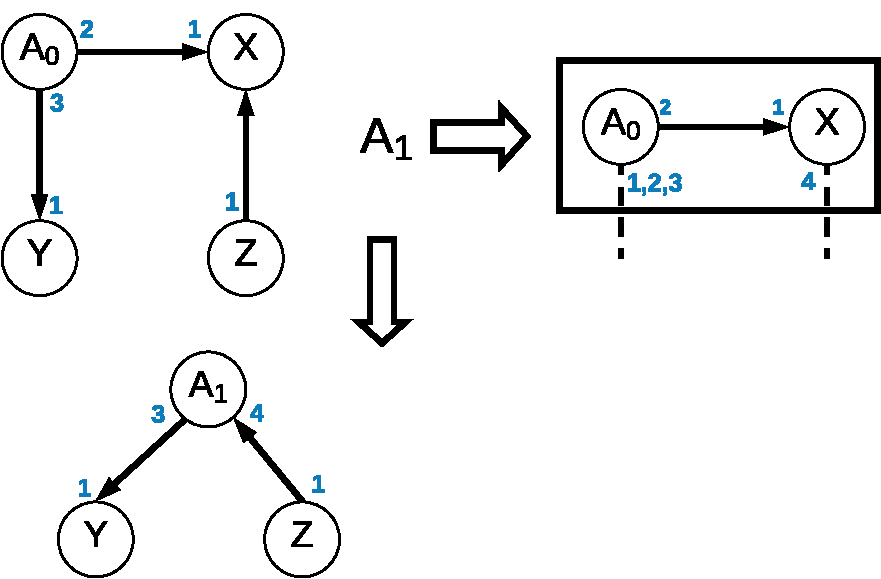
\includegraphics[width=0.6\textwidth]{img/nodeEC}
	\caption{Visualization of equivalence classes of the nodes}
	\label{fig:nodeEC}
\end{figure}

Therefore, the inner nodes of a nonterminal node rule are numbered consecutively, where we call the numbers of the inner nodes equivalence classes. Thus, incident edges of a nonterminal symbol are labeled with the equivalence class of the inner node to which the edge was incident before its replacement. 

If the node is a terminal, it has equivalence class 1. To simplify matters, the equivalence classes for terminals are often not displayed in the representations.

\subsection*{Equivalence classes for edges}
If multiple edges are replaced by one nonterminal hyperedge, the information about which of the inner edges were incident to which node must still be available.

In Fig.~\ref{fig:edgeEC} we see a replacement of several edges by a hyperedge. If there were no equivalence classes for the edges, one would not know to which node the inner edge with the label d must be incident. No information about the direction of the edge ends is required, so the hyperedge is undirected. Therefore, the edge ends are numbered, where we call the numbers equivalence classes for edges.
\begin{figure}[h]
	\centering
	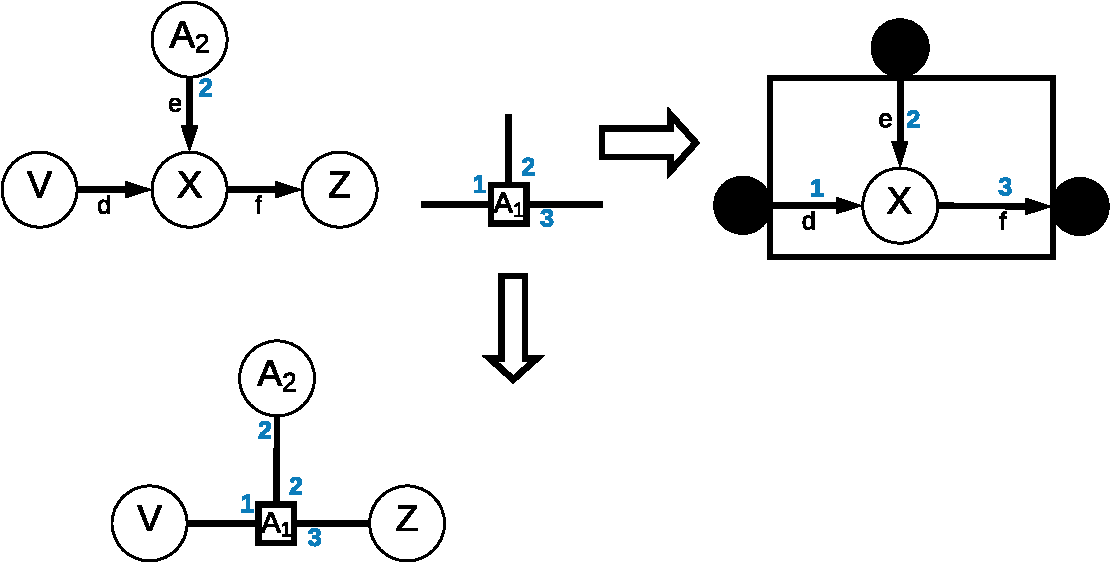
\includegraphics[width=0.8\textwidth]{img/edgeEC}
	\caption{Visualization of equivalence classes of the edges}
	\label{fig:edgeEC}
\end{figure}

If two internal edges contain the same information (same direction, label and incident with the same equivalence class at the inner node), the edge ends have the same equivalence class. If there is now another incoming edge with label "e" and the equivalence classes are the same as the other edge with label "e", it can be replaced with the same digram, since the new edge also gets the edge equivalence class "2".


In the special case that an edge is not a hyperedge, the edge has two ends. Thus the edge can be represented normally and the equivalence classes 1 and 2 can be represented over one direction of the edge, see Fig.~\ref{fig:edgeECsimple}. The end, which is incident to the start node, has the equivalence class 1 and the end, which is incident to the end node, has the equivalence class 2.
\begin{figure}[h]
	\centering
	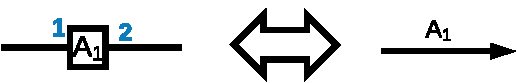
\includegraphics[width=0.4\textwidth]{img/edgeEC_simple}
	\caption{Simplified representation of an edge with equivalence classes}
	\label{fig:edgeECsimple}
\end{figure}


\asd{If a Digram has only one external node, only one edge end is required. Since each edge must have 2 ends, an edge is inserted where both ends point to the desired node. An example can be seen in Figure 3 from the document "All different Types of digram Types from Maneth and Peternek".}
\subsection*{Parameters}

It may make sense to allow a parameter for a digram. If a pattern occurs again and again, but the node label at a node, for example, varies again and again, this can be combined into a digram and the node label can be stored as a parameter. This can significantly increase the number of occurrences found.

Any internal information of a digram rule can be parameterized. Thus the edge direction, equivalence classes, nodes/edge labels can be parameterized.

In addition, external elements can possibly become internal elements and the varying information can be parameterized. Thus, for example, the external node in the adjacency digram (Section~\ref{sec:adjacencyDigram}) becomes an internal node and its node label becomes a parameter.
It should be noted that the modified form of adjacency digram will be a double application of basic digrams (Section~\ref{sec:basicDigram}). But this digram (Section~\ref{sec:adjacencyDigram}) will probably not be created only with basic digrams, because the middle node label varies and therefore no frequently occurring basic digram can be found. This characteristic will probably also occur with other variations.




\section{Basic digram}
\label{sec:basicDigram}


The basic digram (Fig.~\ref{fig:basicDigram}) consists of two adjacent nodes and the edge that connects these nodes. Thus, two adjacent nodes and the incident edge can be replaced by one nonterminal node. Each node is assigned with an equivalence class. For each occurrence the node labels (x and y), the edge label (e), and the equivalence classes (i and j) of the inner edge must match as defined in the rule.

\begin{figure}[h]
	\centering
	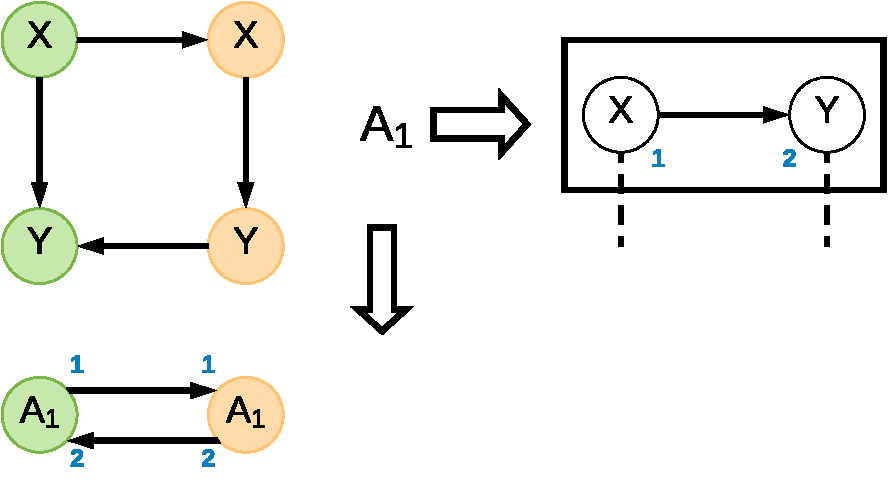
\includegraphics[width=0.6\textwidth]{img/basicDigram}
	\caption{Application of a replacement of a basic digram}
	\label{fig:basicDigram}
\end{figure}

\section{Circle digram}
\label{sec:circleDigram}



The circle digram (Fig.~\ref{fig:circleDigram}) contains a node and an edge, which is a self-cycle of the node. The node and the edge are replaced by a nonterminal node. For each occurrence the node label x, the edge label e, and the equivalence classes (i and j) of the edge must match as defined in the rule.

\begin{figure}[h]
	\centering
	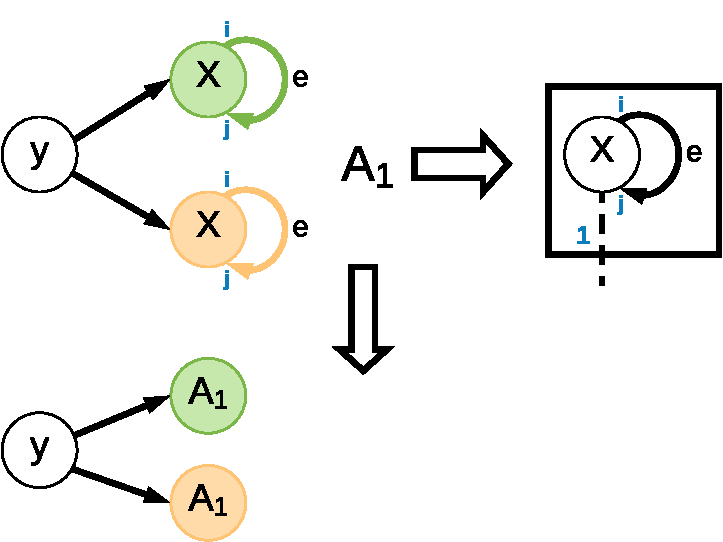
\includegraphics[width=0.6\textwidth]{img/circleDigram}
	\caption{Application of a replacement of a circle digram}
	\label{fig:circleDigram}
\end{figure}



\section{Adjacency digram}
\label{sec:adjacencyDigram}



The adjacency digram (Fig.~\ref{fig:adjacencyDigram}) is formed by two nodes which both have a common adjacency node U. Thus, the adjacency digram contains the two nodes and the two edges that are incident to the node U. This digram can be replaced by a nonterminal node and an edge from the nonterminal node to the node U. Each inner node and the external node is assigned an equivalence class.
The incident edges must have the same equivalence classes k at the external node, but the equivalence class can differ for each occurrence of the digram. This is necessary because the two internal edges are replaced by one edge so that only one equivalence class can be assigned to the new edge at one end.

\begin{figure}[h]
	\centering
	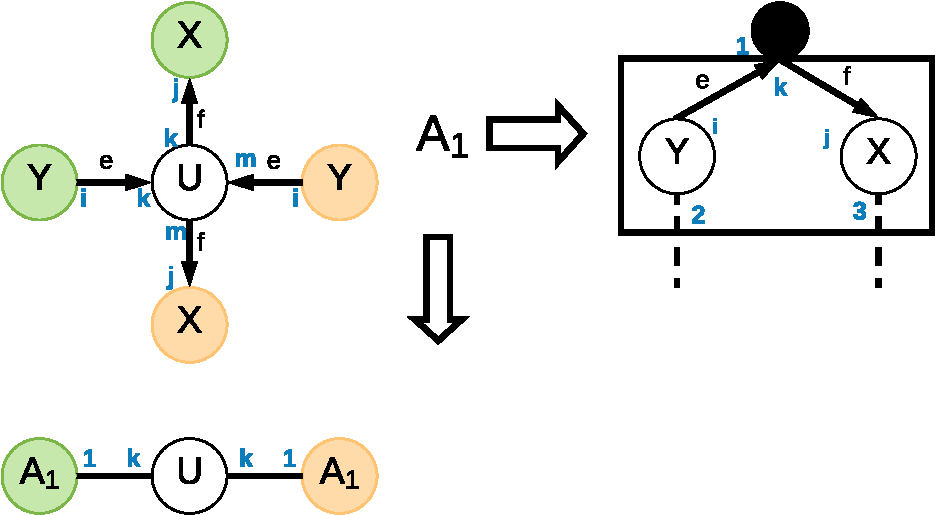
\includegraphics[width=0.5\textwidth]{img/adjacencyDigram}
	\caption{Application of a replacement of an adjacency digram}
	\label{fig:adjacencyDigram}
\end{figure}


\section{Node association digram}
\label{sec:associationDigram}


The node association digram (Fig.~\ref{fig:nodeAssociationDigram}) is a generalization of an adjacency digram.
This digram consists of two nodes, which are combined to one node. Each node is assigned with an equivalence class.
In this way, frequently occurring nodes are replaced by a nonterminal node and these do not have to be adjacent. However, this replacement increases the number of incident edges per node, since the new node unites the incident edges of the old nodes.

\begin{figure}[h]
	\centering
	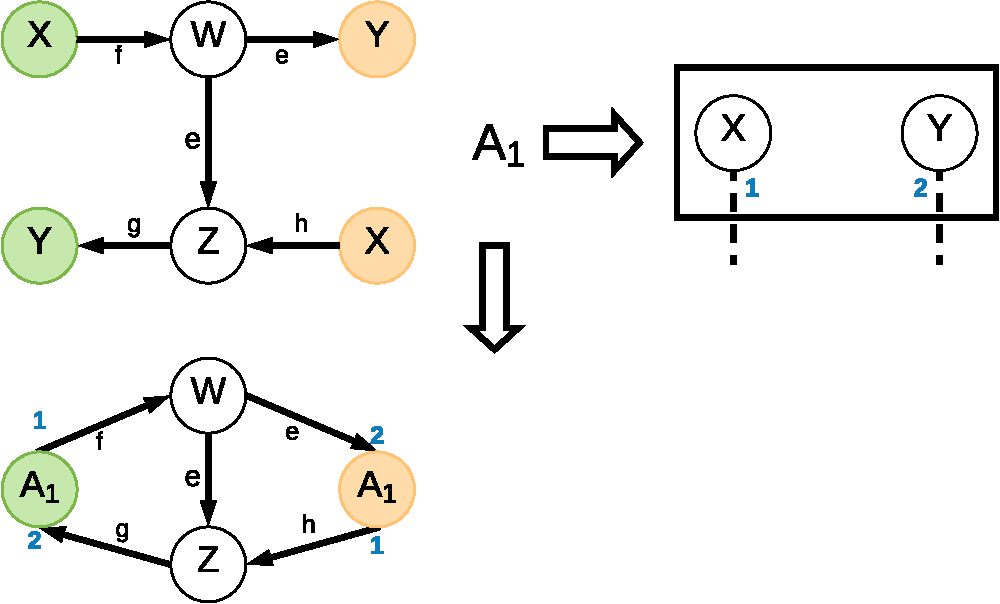
\includegraphics[width=0.5\textwidth]{img/nodeAssociationDigram}
	\caption{Application of a replacement of a node association digram}
	\label{fig:nodeAssociationDigram}
\end{figure}


\section{Clique digram}
\label{sec:cliqueDigram}


The clique digram (Fig.~\ref{fig:cliqueDigram}) is a generalization of an adjacency digram.
This clique digram consists of two nodes, which are strongly connected. The occurrences are replaced by a node. Each node is assigned an equivalence class. The digram can also be generated by applying the basic digram (Chapter~\ref{sec:basicDigram}) and then the circle digram( Chapter~\ref{sec:circleDigram}). \asd{However, the Digram Clique offers only one advantage if all edges of the clique have the same label. Then the advantage is that the edges in the Digram do not have to be saved in the rule call, because it is clear that for every inner node from one node to every other inner node an edge exists. If the edges now have different labels, the labels must be able to be assigned to the edges again, so that the clique digram no longer offers any advantage.} If one of the two nodes is already a nonterminal symbol, the other node should be strongly connected to each inner node. 

\begin{figure}[h]
	\centering
	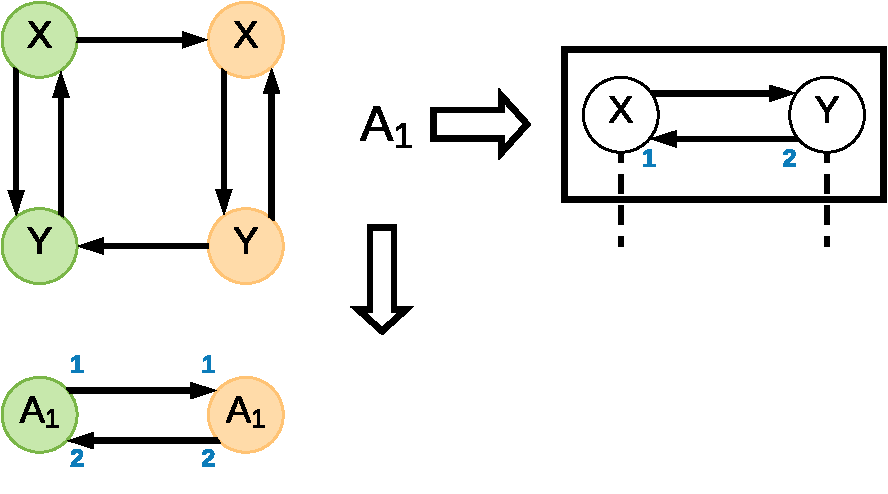
\includegraphics[width=0.5\textwidth]{img/cliqueDigram}
	\caption{Application of a replacement of a clique digram}
	\label{fig:cliqueDigram}
\end{figure}
As the digram can be reproduced by other digrams, this type of digram is not taken into account when searching for and replacing the most frequent digram, but possibly only when pruning the existing rules to more efficient rules.



\section{Basic edge digram}
\label{sec:basicEdgeDigram}


The basic edge digram (Fig.~\ref{fig:basicEdgeDigram}) is the opposite of the basic digram.
Here, two edges and a node, where both edges are incident to the node, are replaced by one edge. The directions of the edges and the edge labels must be the same in all occurrences. In addition, the equivalence classes at the inner node must match. Furthermore, the inner node must not have any other incident edges than the two internal edges. 

\begin{figure}[h]
	\centering
	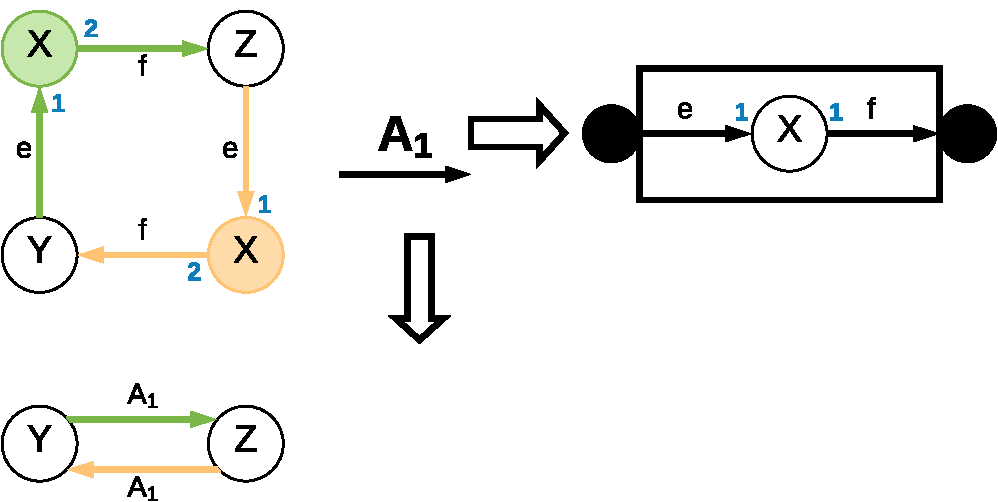
\includegraphics[width=0.7\textwidth]{img/basicEdgeDigram}
	\caption{Application of a replacement of a basic edge digram}
	\label{fig:basicEdgeDigram}
\end{figure}


\subsection*{Incedent edges to an inner node}
\label{sec:incedentEdges}

The basic edge digram described above only works if the inner node has no other incident edges. This is probably rarely the case in reality, so the rule has to be extended so that there can be an arbitrary number of nodes be incident to the edge.

I currently have two approaches, both of which have their downsides.
\\\\
Case 1: All incident edges are transformed into a hyper edge

The two internal edges (with the labels e and f) have been transformed into a simple edge $A_1$ so far. In addition, all incident edges of the node x are now added to the new edge $A_1$, so that the edge is a hyper edge if there are external incident edges. However, the information (edge direction, edge label and equivalence class to the internal node) of the individual edges must not be lost. 

Figure~\ref{fig:incedentEdges1} illustrates how the edge directions for all external incident edges can be handled. Therefore incoming edges get the equivalence class 3 and outgoing edges get the equivalence class 4. 

\begin{figure}[h]
	\centering
	\includegraphics[width=0.8\textwidth]{img/edgeDigram_params}
	\caption{Application of a replacement of a basic edge digram with incident edges to the internal node}
	\label{fig:incedentEdges1}
\end{figure}

Thus, the edge label and the equivalence class must be parameterized for each external incident edge. You must also make sure that the parameters can be assigned to the correct edge end of the hyper edge. Since the number of external incident edges is arbitrary, the number of parameters can be arbitrarily large. 

In this case, the parameter must therefore be included:
\begin{itemize}
\item W: Label is g; equivalence class is 2
\item U: Label is h; equivalence class is 3
\item V: Label is d; equivalence class is 1
\item Which end contained which labels
\end{itemize}
\asd{These parameters could then be saved as extended edge labels, for example. So the label would not only contain the nonterminal name but also the parameters. If the edge is to be replaced in another digram, the complete label must match so that the parameters match.}


Case 2: External incident edges of the internal node become incident edges of an external node. 

All external incident edges to X (see Fig.~\ref{fig:incedentEdges2}) become incident to the external nodes, which is the start node of the edge (in this case Y). This changes the number of incident edges to Y, where you have to be able to distinguish which of the edges were incident to X before. Therefore, the equivalence classes in Y must be changed so that this is possible.

Thus an existing node is changed and also the new nonterminal edge. Therefore, two persisting elements are changed by the replacement of the digram, whereby this type of digram turns the graph into a non context-free grammar. Furthermore it should be clarified how in node Y the label is not lost, but the reference to the rule $A_1$, which is normally represented by the label of the element, is still present. Additionally, by changing external nodes, the subsequent compression is made more difficult, because parts of the occurrences of Y are modified and are therefore no longer synonymous with unmodified Y occurrences.

\begin{figure}[h]
	\centering
	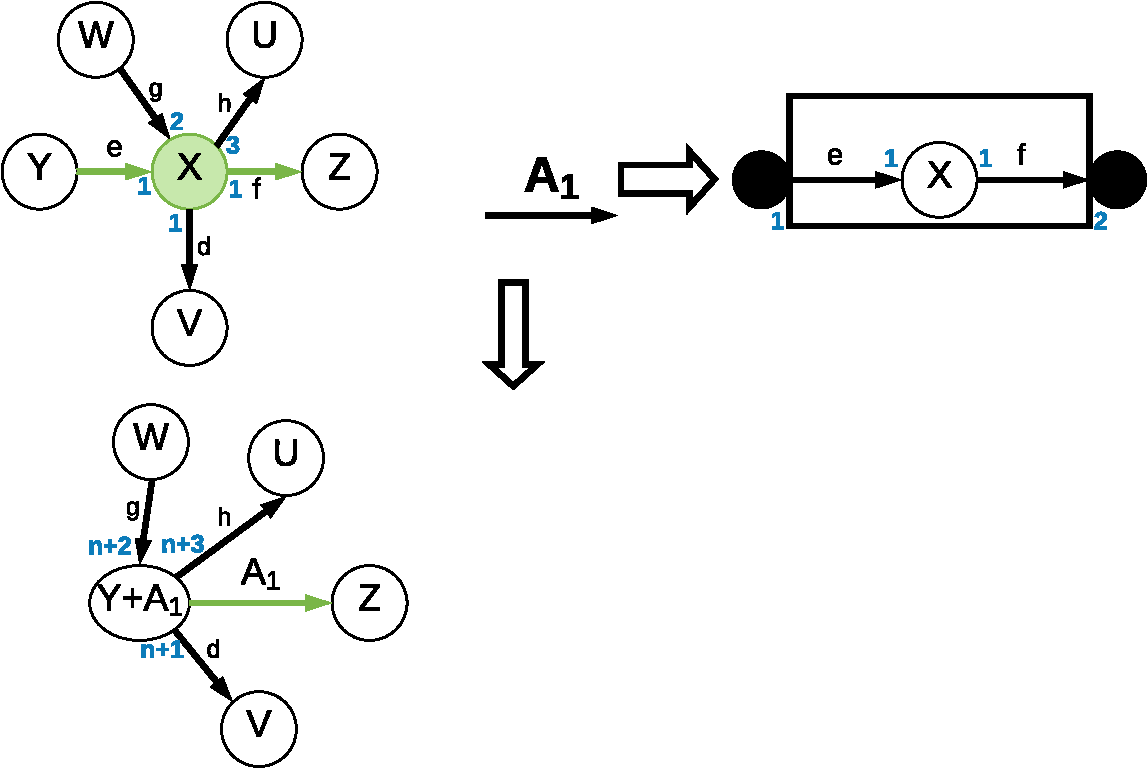
\includegraphics[width=0.8\textwidth]{img/edgeDigram_extern}
	\caption{Application of a replacement of a basic edge digram with incident edges to the internal node. 'n' is the number of different equivalence classes of Y before substitution}
	\label{fig:incedentEdges2}
\end{figure}

\section{Edge association digram}
\label{sec:edgeAssociationDigram}


This edge association digram (Fig.~\ref{fig:edgeAssociationDigram}) combines two adjacent edges to one hyper edge

Here only the two edges are internal elements of the rule. The equivalence classes at the middle external node must be the same. The replacement results in a hyper edge which in turn has equivalence classes of its own. The directions of the edges and the edge labels must be the same in all occurrences.
\begin{figure}[h]
	\centering
	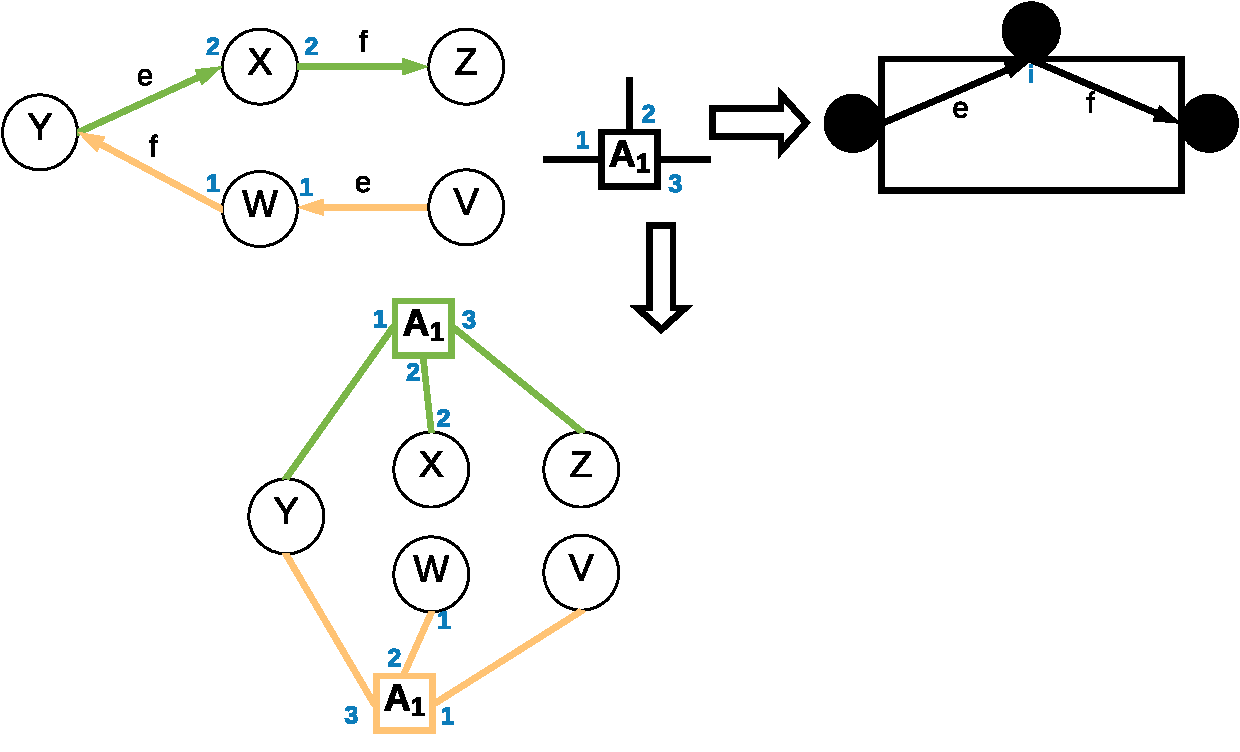
\includegraphics[width=1\textwidth]{img/edgeAssociationDigram}
	\caption{Application of a replacement of an edge association digram}
	\label{fig:edgeAssociationDigram}
\end{figure}

\section{Other digram types}
All other digram types from Maneth can be adopted analogously. First, you should definitely determine how incident edges can be treated to internal nodes (Section.~\ref{sec:incedentEdges}), since this case also occurs in the other types.


\pagebreak
\section{Combine substitutions of different digram types}
In this section different digram types were presented, but the question arises whether all digram types can be combined. If a digram type is applied to a graph, the graph will be changed to a hyperedge, for example. If now other digram types are to be applied, it must not come to cases by the changed graph that something goes wrong with the further replacements. Thus it is considered here whether all Digram types are compatible with all others.

\section{Search for Digram occurrences}


%\printbibliography








\end{document}